\documentclass[a4paper,10pt,twoside]{article}

\usepackage[top=1in, bottom=1in, left=1in, right=1in]{geometry}
\usepackage[utf8]{inputenc}
\usepackage[spanish,es-ucroman,es-noquoting]{babel}
\usepackage{setspace}
\usepackage{fancyhdr}
\usepackage{lastpage}
\usepackage{amsmath}
\usepackage{amsfonts}
\usepackage{verbatim}
\usepackage{float}
\usepackage{graphicx}
\usepackage{subcaption}
\usepackage{algorithmic}
\usepackage{amssymb}
\usepackage{url}
\usepackage{moreverb}


% Evita que el documento se estire verticalmente para ocupar
% el espacio vacío en cada página.
\raggedbottom


%%%%%%%%%% Configuración de Fancyhdr - Inicio %%%%%%%%%%
\pagestyle{fancy}
\thispagestyle{fancy}
\lhead{Trabajo Práctico 2, Organización del Computador II}
\rhead{Capra, Lovisolo, Petaccio}
\renewcommand{\footrulewidth}{0.4pt}
\cfoot{\thepage /\pageref{LastPage}}

\fancypagestyle{caratula} {
   \fancyhf{}
   \cfoot{\thepage /\pageref{LastPage}}
   \renewcommand{\headrulewidth}{0pt}
   \renewcommand{\footrulewidth}{0pt}
}
%%%%%%%%%% Configuración de Fancyhdr - Fin %%%%%%%%%%

\newcommand{\real}{\mathbb{R}}

\begin{document}


%%%%%%%%%%%%%%%%%%%%%%%%%%%%%%%%%%%%%%%%%%%%%%%%%%%%%%%%%%%%%%%%%%%%%%%%%%%%%%%
%% Carátula                                                                  %%
%%%%%%%%%%%%%%%%%%%%%%%%%%%%%%%%%%%%%%%%%%%%%%%%%%%%%%%%%%%%%%%%%%%%%%%%%%%%%%%


\thispagestyle{caratula}

\begin{center}


\includegraphics[height=2cm]{DC.png} 
\hfill

\includegraphics[height=2cm]{UBA.jpg} 

\vspace{2cm}

Departamento de Computación,\\
Facultad de Ciencias Exactas y Naturales,\\
Universidad de Buenos Aires

\vspace{2cm}

\begin{spacing}{1}
\begin{Huge}

Reconocimiento de Dígitos Manuscritos\\
con la Descomposición en Valores Singulares

\end{Huge}
\end{spacing}

\vspace{2cm}

Trabajo Práctico 1, \\
Métodos Numéricos, \\
Primer Cuatrimestre de 2013

\vspace{3cm}

\begin{tabular}{|c|c|c|}
\hline
Apellido y Nombre & LU & E-mail\\
\hline
María Candela Capra Coarasa & 234/11 & canduh\_27@hotmail.com\\
Leandro Lovisolo            & 645/11 & leandro@leandro.me\\
Lautaro José Petaccio       & 443/11 & lausuper@gmail.com\\
\hline
\end{tabular}

\end{center}

\vspace{3cm}

\textbf{Resumen:} \\
Se implementa un método de reconocimiento de dígitos manuscritos basado en la descomposición en valores singulares, y se analizan empíricamente los parámetros principales del método.

\textbf{Palabras clave:}
OCR, dígitos manuscritos, reconocimiento, SVD, algoritmo QR.

\newpage


%%%%%%%%%%%%%%%%%%%%%%%%%%%%%%%%%%%%%%%%%%%%%%%%%%%%%%%%%%%%%%%%%%%%%%%%%%%%%%%
%% Índice                                                                    %%
%%%%%%%%%%%%%%%%%%%%%%%%%%%%%%%%%%%%%%%%%%%%%%%%%%%%%%%%%%%%%%%%%%%%%%%%%%%%%%%


\tableofcontents

\newpage


%%%%%%%%%%%%%%%%%%%%%%%%%%%%%%%%%%%%%%%%%%%%%%%%%%%%%%%%%%%%%%%%%%%%%%%%%%%%%%%
%% Introducción Teórica                                                      %%
%%%%%%%%%%%%%%%%%%%%%%%%%%%%%%%%%%%%%%%%%%%%%%%%%%%%%%%%%%%%%%%%%%%%%%%%%%%%%%%


\section{Introducción Teórica}

Definimos a continuación un conjunto de conceptos utilizados a lo largo de este trabajo.


\subsection{Matriz de covarianza}

Sea $\{x_1, \ldots x_n\}$ un conjunto de variables aleatorias, y sean $\sigma_{x_i, x_j}$ sus respectivas covarianzas (con $1 \leq i, j \leq n$). 

Definimos la matriz de covarianza de $\{x_1, \ldots x_n\}$ de la siguiente manera:

$$
  \begin{pmatrix}
    \sigma x_1,x_1 & \sigma x_1,x_2 & \cdots & \sigma x_1,x_n \\
    \sigma x_2,x_1 & \sigma x_2,x_2 & \cdots & \sigma x_2,x_n \\
    \vdots  & \vdots  & \ddots & \vdots  \\
    \sigma x_n,x_1 & \sigma x_n,x_2 & \cdots & \sigma x_n,x_n \\
  \end{pmatrix}
$$


\subsection{Transformación característica}

Para $i = 1,\ldots, n$, sea $x_i \in \real^{m}$ la $i$-\'esima imagen de nuestra base de datos almacenada por filas en un vector, y sea $\mu = (x_1 + \ldots + x_n)/n$ el promedio de las im\'agenes. Definimos $X\in\real^{n\times m}$ como la matriz que contiene en la $i$-\'esima fila al vector $(x_i - \mu)^{t}/\sqrt{n-1}$, y

$$X=U \Sigma V^t$$

a su descomposici\'on en valores singulares, con $U\in\real^{n\times n}$ y $V\in\real^{m\times m}$ matrices ortogonales, y $\Sigma\in\real^{n\times m}$ la matriz diagonal conteniendo en la posici\'on $(i,i)$ al $i$-\'esimo valor singular $\sigma_i$.
Siendo $v_i$ la columna $i$ de $V$, definimos para $i = 1,\ldots,n$ la \textsl{transformaci\'on caracter\'istica} del d\'igito $x_{i}$ como el vector $\mathbf{tc}(x_i) = (v_1^t\, x_i, v_2^t\, x_i,\ldots,v_k^t\, x_i) \in\real^k$, donde $k \in\{1,\ldots,m\}$ es un par\'ametro de la implementaci\'on.


\subsection{Algoritmo QR}

Describimos a continuación el algoritmo empleado en este trabajo para aproximar los autovectores necesarios para computar la transformación característica.

\begin{algorithmic}
  \STATE Input($A$)
  \STATE $A_1$ $\leftarrow$ $A$
  \WHILE{\textbf{not} CondiciónDeParada()}
    \STATE $Q_k$, $R_k$ $\leftarrow$ FactorizaciónQR($A_k$)
    \STATE $A_{k+1} \leftarrow R_k \times Q_k$
  \ENDWHILE
  \STATE Output($A_{k+1}$, $Q_k$)
\end{algorithmic}


%%%%%%%%%%%%%%%%%%%%%%%%%%%%%%%%%%%%%%%%%%%%%%%%%%%%%%%%%%%%%%%%%%%%%%%%%%%%%%%
%% Desarrollo                                                                %%
%%%%%%%%%%%%%%%%%%%%%%%%%%%%%%%%%%%%%%%%%%%%%%%%%%%%%%%%%%%%%%%%%%%%%%%%%%%%%%%


\section{Desarrollo}


\subsection{Método}

Dado un conjunto de $n$ imágenes de entrenamiento $\{x_1, \ldots x_n\}$ con $x_i \in \real^{m \times m}$ y una imagen $x$ que no pertenece al conjunto anterior, queremos identificar el dígito $d$ representado por la imagen $x$.

Sean $X_0, \ldots X_9$ los conjuntos de imágenes de entrenamiento etiquetadas con los dígitos $0, \ldots 9$, respectivamente, y sea $x_j^i \in X_i$ la $j$-ésima imagen etiquetada con el dígito $i$.

Definimos la \textit{transformada característica media} del dígito $i$ como:

$$
tc_i = \frac{\sum_{j=1}^{|X_i|}{tc(x_j^i)}}
            {|X_i|}
$$

Hallamos el dígito $d$, representado por la imagen $x$, de la siguiente manera:

$$
d = \min_{i} || tc_i - tc(x) ||_2
$$

Es decir, identificamos el dígito correspondiente a la imagen $x$ como el dígito cuya transformada característica media se encuentra a menor distancia euclídea de la transformada característica de la imagen $x$.


\subsection{Aproximación de autovectores}

Aplicamos el algoritmo QR para aproximar los autovectores de la matriz de covarianza de las imágenes de entrenamiento $\{x_1, \ldots x_n\}$. 

Como criterio de parada, empleamos una cota superior para la suma del módulo de los elementos por debajo de la diagonal principal de la matriz $A_{k+1}$ obtenida luego de la $k$-ésima iteración del algoritmo.

Implementamos un método de descomposición QR utilizando transformaciones de Householder. La implementación inicial de este método empleaba transformaciones de Givens, pero esta técnica resultó demasiado lenta, por lo que luego fue reemplazado por la implementación actual basada en reflectores.

A continuación, tomamos la matriz diagonal $A$ y la matriz ortogonal $R$ obtenidas de la salida del algoritmo QR. Recordemos que los elementos $a_ii$ de la diagonal de la matriz $A$ aproximan los autovalores de la matriz de covarianza, mientras que la $i$-ésima columna de la matriz $Q$ contiene una aproximación al autovector asociado al autovalor $a_ii$. Para terminar, reordenamos los autovectores por autovalor asociado, de forma decreciente.


\subsection{Experimentos realizados}

Realizamos una serie de experimentos haciendo variar la cantidad de coeficientes principales $k$ y la cantidad de iteraciones $i$ del algoritmo QR, de manera de poder hallar las configuraciones que produzcan las mejores tasas de aciertos posibles.

En todos los experimentos se utilizó la base de datos de dígitos manuscritos MNIST\footnote{http://yann.lecun.com/exdb/mnist/}. Salvo en un experimento en particular, se generó en cada caso la matriz de covarianza empleando los 60,000 ejemplares de entrenamiento, y se computó la tasa de aciertos identificando los 10,000 ejemplares de prueba.


\subsubsection{Tasa de acierto en función de número de iteraciones del algoritmo QR}

Llevamos a cabo 50 iteraciones del algoritmo QR, tomamos los autovectores aproximados en cada iteración del algoritmo y los utilizamos para computar la tasa de aciertos del método para $k = 600$.


\subsubsection{Tasa de acierto en función de cantidad de coeficientes principales}

Evaluamos el método para valores de $k = 1, \ldots 100$, utilizando una cota de error $e = 1000$ como criterio de parada del algoritmo QR.


\subsubsection{Tasa de acierto en función de cantidad de imágenes de entrenamiento}

Evaluamos la tasa de aciertos para $k = 40$ y cota de error $e = 1000$, utilizando subconjuntos del cuerpo de entrenamiento de distintos tamaños.


%%%%%%%%%%%%%%%%%%%%%%%%%%%%%%%%%%%%%%%%%%%%%%%%%%%%%%%%%%%%%%%%%%%%%%%%%%%%%%%
%% Resultados                                                                %%
%%%%%%%%%%%%%%%%%%%%%%%%%%%%%%%%%%%%%%%%%%%%%%%%%%%%%%%%%%%%%%%%%%%%%%%%%%%%%%%


\section{Resultados}


Presentamos a continuación los resultados de los experimentos explicados anteriormente.

\begin{figure}[H]
  \centering
  % GNUPLOT: LaTeX picture with Postscript
\begingroup
  \makeatletter
  \providecommand\color[2][]{%
    \GenericError{(gnuplot) \space\space\space\@spaces}{%
      Package color not loaded in conjunction with
      terminal option `colourtext'%
    }{See the gnuplot documentation for explanation.%
    }{Either use 'blacktext' in gnuplot or load the package
      color.sty in LaTeX.}%
    \renewcommand\color[2][]{}%
  }%
  \providecommand\includegraphics[2][]{%
    \GenericError{(gnuplot) \space\space\space\@spaces}{%
      Package graphicx or graphics not loaded%
    }{See the gnuplot documentation for explanation.%
    }{The gnuplot epslatex terminal needs graphicx.sty or graphics.sty.}%
    \renewcommand\includegraphics[2][]{}%
  }%
  \providecommand\rotatebox[2]{#2}%
  \@ifundefined{ifGPcolor}{%
    \newif\ifGPcolor
    \GPcolorfalse
  }{}%
  \@ifundefined{ifGPblacktext}{%
    \newif\ifGPblacktext
    \GPblacktexttrue
  }{}%
  % define a \g@addto@macro without @ in the name:
  \let\gplgaddtomacro\g@addto@macro
  % define empty templates for all commands taking text:
  \gdef\gplbacktext{}%
  \gdef\gplfronttext{}%
  \makeatother
  \ifGPblacktext
    % no textcolor at all
    \def\colorrgb#1{}%
    \def\colorgray#1{}%
  \else
    % gray or color?
    \ifGPcolor
      \def\colorrgb#1{\color[rgb]{#1}}%
      \def\colorgray#1{\color[gray]{#1}}%
      \expandafter\def\csname LTw\endcsname{\color{white}}%
      \expandafter\def\csname LTb\endcsname{\color{black}}%
      \expandafter\def\csname LTa\endcsname{\color{black}}%
      \expandafter\def\csname LT0\endcsname{\color[rgb]{1,0,0}}%
      \expandafter\def\csname LT1\endcsname{\color[rgb]{0,1,0}}%
      \expandafter\def\csname LT2\endcsname{\color[rgb]{0,0,1}}%
      \expandafter\def\csname LT3\endcsname{\color[rgb]{1,0,1}}%
      \expandafter\def\csname LT4\endcsname{\color[rgb]{0,1,1}}%
      \expandafter\def\csname LT5\endcsname{\color[rgb]{1,1,0}}%
      \expandafter\def\csname LT6\endcsname{\color[rgb]{0,0,0}}%
      \expandafter\def\csname LT7\endcsname{\color[rgb]{1,0.3,0}}%
      \expandafter\def\csname LT8\endcsname{\color[rgb]{0.5,0.5,0.5}}%
    \else
      % gray
      \def\colorrgb#1{\color{black}}%
      \def\colorgray#1{\color[gray]{#1}}%
      \expandafter\def\csname LTw\endcsname{\color{white}}%
      \expandafter\def\csname LTb\endcsname{\color{black}}%
      \expandafter\def\csname LTa\endcsname{\color{black}}%
      \expandafter\def\csname LT0\endcsname{\color{black}}%
      \expandafter\def\csname LT1\endcsname{\color{black}}%
      \expandafter\def\csname LT2\endcsname{\color{black}}%
      \expandafter\def\csname LT3\endcsname{\color{black}}%
      \expandafter\def\csname LT4\endcsname{\color{black}}%
      \expandafter\def\csname LT5\endcsname{\color{black}}%
      \expandafter\def\csname LT6\endcsname{\color{black}}%
      \expandafter\def\csname LT7\endcsname{\color{black}}%
      \expandafter\def\csname LT8\endcsname{\color{black}}%
    \fi
  \fi
  \setlength{\unitlength}{0.0500bp}%
  \begin{picture}(7678.00,5280.00)%
    \gplgaddtomacro\gplbacktext{%
      \colorrgb{0.00,0.00,0.00}%
      \put(860,640){\makebox(0,0)[r]{\strut{}81.5}}%
      \colorrgb{0.00,0.00,0.00}%
      \put(860,1448){\makebox(0,0)[r]{\strut{}81.6}}%
      \colorrgb{0.00,0.00,0.00}%
      \put(860,2256){\makebox(0,0)[r]{\strut{}81.7}}%
      \colorrgb{0.00,0.00,0.00}%
      \put(860,3063){\makebox(0,0)[r]{\strut{}81.8}}%
      \colorrgb{0.00,0.00,0.00}%
      \put(860,3871){\makebox(0,0)[r]{\strut{}81.9}}%
      \colorrgb{0.00,0.00,0.00}%
      \put(860,4679){\makebox(0,0)[r]{\strut{}82}}%
      \colorrgb{0.00,0.00,0.00}%
      \put(980,440){\makebox(0,0){\strut{}0}}%
      \colorrgb{0.00,0.00,0.00}%
      \put(2247,440){\makebox(0,0){\strut{}10}}%
      \colorrgb{0.00,0.00,0.00}%
      \put(3515,440){\makebox(0,0){\strut{}20}}%
      \colorrgb{0.00,0.00,0.00}%
      \put(4782,440){\makebox(0,0){\strut{}30}}%
      \colorrgb{0.00,0.00,0.00}%
      \put(6050,440){\makebox(0,0){\strut{}40}}%
      \colorrgb{0.00,0.00,0.00}%
      \put(7317,440){\makebox(0,0){\strut{}50}}%
      \colorrgb{0.00,0.00,0.00}%
      \put(160,2659){\rotatebox{90}{\makebox(0,0){\strut{}Aciertos [\%]}}}%
      \colorrgb{0.00,0.00,0.00}%
      \put(4148,140){\makebox(0,0){\strut{}$i$}}%
      \csname LTb\endcsname%
      \put(4148,4979){\makebox(0,0){\strut{}Tasa de aciertos en función de número de iteraciones $i$}}%
    }%
    \gplgaddtomacro\gplfronttext{%
    }%
    \gplbacktext
    \put(0,0){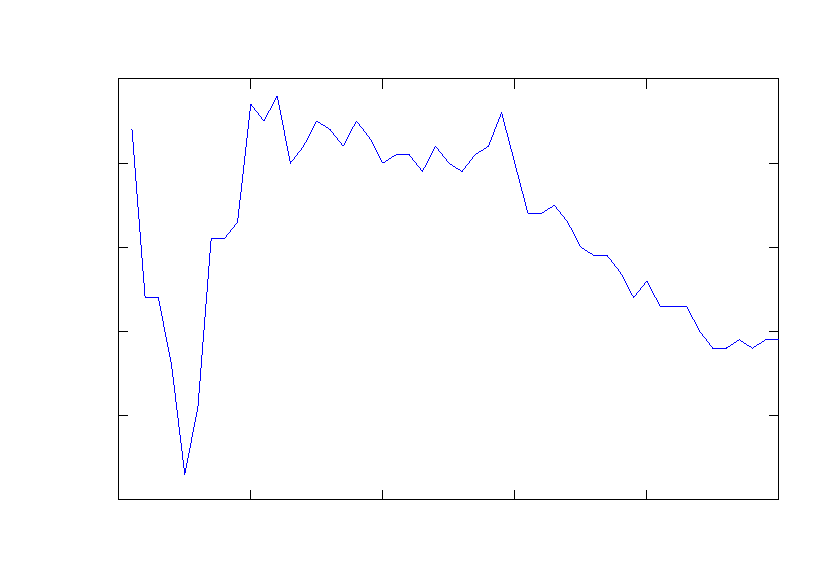
\includegraphics{tasas-vs-iteraciones}}%
    \gplfronttext
  \end{picture}%
\endgroup

  \caption{Tasa de aciertos en función de número $i$ de iteraciones del algoritmo QR.}
  \label{tasas-vs-iteraciones}
\end{figure}

\begin{figure}[H]
  \centering
  % GNUPLOT: LaTeX picture with Postscript
\begingroup
  \makeatletter
  \providecommand\color[2][]{%
    \GenericError{(gnuplot) \space\space\space\@spaces}{%
      Package color not loaded in conjunction with
      terminal option `colourtext'%
    }{See the gnuplot documentation for explanation.%
    }{Either use 'blacktext' in gnuplot or load the package
      color.sty in LaTeX.}%
    \renewcommand\color[2][]{}%
  }%
  \providecommand\includegraphics[2][]{%
    \GenericError{(gnuplot) \space\space\space\@spaces}{%
      Package graphicx or graphics not loaded%
    }{See the gnuplot documentation for explanation.%
    }{The gnuplot epslatex terminal needs graphicx.sty or graphics.sty.}%
    \renewcommand\includegraphics[2][]{}%
  }%
  \providecommand\rotatebox[2]{#2}%
  \@ifundefined{ifGPcolor}{%
    \newif\ifGPcolor
    \GPcolorfalse
  }{}%
  \@ifundefined{ifGPblacktext}{%
    \newif\ifGPblacktext
    \GPblacktexttrue
  }{}%
  % define a \g@addto@macro without @ in the name:
  \let\gplgaddtomacro\g@addto@macro
  % define empty templates for all commands taking text:
  \gdef\gplbacktext{}%
  \gdef\gplfronttext{}%
  \makeatother
  \ifGPblacktext
    % no textcolor at all
    \def\colorrgb#1{}%
    \def\colorgray#1{}%
  \else
    % gray or color?
    \ifGPcolor
      \def\colorrgb#1{\color[rgb]{#1}}%
      \def\colorgray#1{\color[gray]{#1}}%
      \expandafter\def\csname LTw\endcsname{\color{white}}%
      \expandafter\def\csname LTb\endcsname{\color{black}}%
      \expandafter\def\csname LTa\endcsname{\color{black}}%
      \expandafter\def\csname LT0\endcsname{\color[rgb]{1,0,0}}%
      \expandafter\def\csname LT1\endcsname{\color[rgb]{0,1,0}}%
      \expandafter\def\csname LT2\endcsname{\color[rgb]{0,0,1}}%
      \expandafter\def\csname LT3\endcsname{\color[rgb]{1,0,1}}%
      \expandafter\def\csname LT4\endcsname{\color[rgb]{0,1,1}}%
      \expandafter\def\csname LT5\endcsname{\color[rgb]{1,1,0}}%
      \expandafter\def\csname LT6\endcsname{\color[rgb]{0,0,0}}%
      \expandafter\def\csname LT7\endcsname{\color[rgb]{1,0.3,0}}%
      \expandafter\def\csname LT8\endcsname{\color[rgb]{0.5,0.5,0.5}}%
    \else
      % gray
      \def\colorrgb#1{\color{black}}%
      \def\colorgray#1{\color[gray]{#1}}%
      \expandafter\def\csname LTw\endcsname{\color{white}}%
      \expandafter\def\csname LTb\endcsname{\color{black}}%
      \expandafter\def\csname LTa\endcsname{\color{black}}%
      \expandafter\def\csname LT0\endcsname{\color{black}}%
      \expandafter\def\csname LT1\endcsname{\color{black}}%
      \expandafter\def\csname LT2\endcsname{\color{black}}%
      \expandafter\def\csname LT3\endcsname{\color{black}}%
      \expandafter\def\csname LT4\endcsname{\color{black}}%
      \expandafter\def\csname LT5\endcsname{\color{black}}%
      \expandafter\def\csname LT6\endcsname{\color{black}}%
      \expandafter\def\csname LT7\endcsname{\color{black}}%
      \expandafter\def\csname LT8\endcsname{\color{black}}%
    \fi
  \fi
  \setlength{\unitlength}{0.0500bp}%
  \begin{picture}(7678.00,5280.00)%
    \gplgaddtomacro\gplbacktext{%
      \colorrgb{0.00,0.00,0.00}%
      \put(620,640){\makebox(0,0)[r]{\strut{}30}}%
      \colorrgb{0.00,0.00,0.00}%
      \put(620,1313){\makebox(0,0)[r]{\strut{}40}}%
      \colorrgb{0.00,0.00,0.00}%
      \put(620,1986){\makebox(0,0)[r]{\strut{}50}}%
      \colorrgb{0.00,0.00,0.00}%
      \put(620,2660){\makebox(0,0)[r]{\strut{}60}}%
      \colorrgb{0.00,0.00,0.00}%
      \put(620,3333){\makebox(0,0)[r]{\strut{}70}}%
      \colorrgb{0.00,0.00,0.00}%
      \put(620,4006){\makebox(0,0)[r]{\strut{}80}}%
      \colorrgb{0.00,0.00,0.00}%
      \put(620,4679){\makebox(0,0)[r]{\strut{}90}}%
      \colorrgb{0.00,0.00,0.00}%
      \put(740,440){\makebox(0,0){\strut{}0}}%
      \colorrgb{0.00,0.00,0.00}%
      \put(2055,440){\makebox(0,0){\strut{}20}}%
      \colorrgb{0.00,0.00,0.00}%
      \put(3371,440){\makebox(0,0){\strut{}40}}%
      \colorrgb{0.00,0.00,0.00}%
      \put(4686,440){\makebox(0,0){\strut{}60}}%
      \colorrgb{0.00,0.00,0.00}%
      \put(6002,440){\makebox(0,0){\strut{}80}}%
      \colorrgb{0.00,0.00,0.00}%
      \put(7317,440){\makebox(0,0){\strut{}100}}%
      \colorrgb{0.00,0.00,0.00}%
      \put(160,2659){\rotatebox{90}{\makebox(0,0){\strut{}Aciertos [\%]}}}%
      \colorrgb{0.00,0.00,0.00}%
      \put(4028,140){\makebox(0,0){\strut{}$k$}}%
      \csname LTb\endcsname%
      \put(4028,4979){\makebox(0,0){\strut{}Tasa de aciertos en función de cantidad de coeficientes principales $k$}}%
    }%
    \gplgaddtomacro\gplfronttext{%
    }%
    \gplbacktext
    \put(0,0){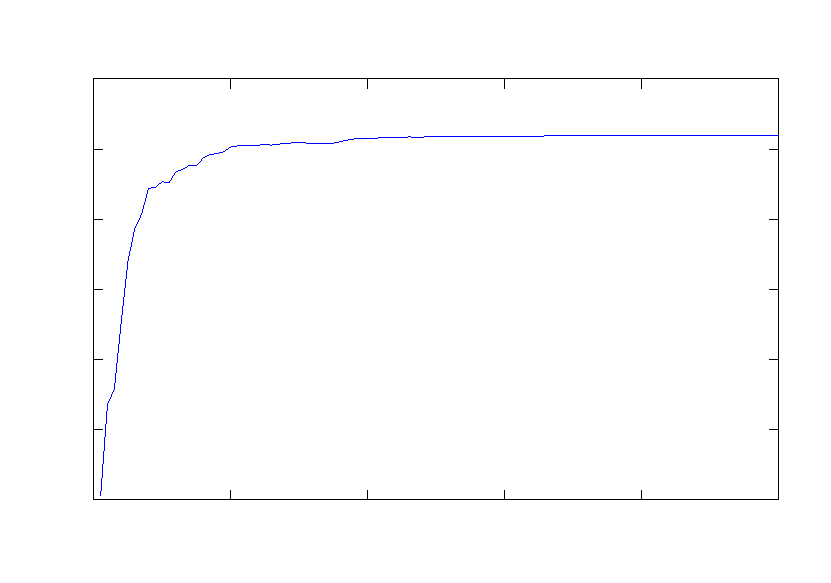
\includegraphics{tasas-vs-k}}%
    \gplfronttext
  \end{picture}%
\endgroup

  \caption{Tasa de aciertos en función de número de coeficientes principales $k$.}
  \label{tasas-vs-k}
\end{figure}

\begin{figure}[H]
  \centering
  % GNUPLOT: LaTeX picture with Postscript
\begingroup
  \makeatletter
  \providecommand\color[2][]{%
    \GenericError{(gnuplot) \space\space\space\@spaces}{%
      Package color not loaded in conjunction with
      terminal option `colourtext'%
    }{See the gnuplot documentation for explanation.%
    }{Either use 'blacktext' in gnuplot or load the package
      color.sty in LaTeX.}%
    \renewcommand\color[2][]{}%
  }%
  \providecommand\includegraphics[2][]{%
    \GenericError{(gnuplot) \space\space\space\@spaces}{%
      Package graphicx or graphics not loaded%
    }{See the gnuplot documentation for explanation.%
    }{The gnuplot epslatex terminal needs graphicx.sty or graphics.sty.}%
    \renewcommand\includegraphics[2][]{}%
  }%
  \providecommand\rotatebox[2]{#2}%
  \@ifundefined{ifGPcolor}{%
    \newif\ifGPcolor
    \GPcolorfalse
  }{}%
  \@ifundefined{ifGPblacktext}{%
    \newif\ifGPblacktext
    \GPblacktexttrue
  }{}%
  % define a \g@addto@macro without @ in the name:
  \let\gplgaddtomacro\g@addto@macro
  % define empty templates for all commands taking text:
  \gdef\gplbacktext{}%
  \gdef\gplfronttext{}%
  \makeatother
  \ifGPblacktext
    % no textcolor at all
    \def\colorrgb#1{}%
    \def\colorgray#1{}%
  \else
    % gray or color?
    \ifGPcolor
      \def\colorrgb#1{\color[rgb]{#1}}%
      \def\colorgray#1{\color[gray]{#1}}%
      \expandafter\def\csname LTw\endcsname{\color{white}}%
      \expandafter\def\csname LTb\endcsname{\color{black}}%
      \expandafter\def\csname LTa\endcsname{\color{black}}%
      \expandafter\def\csname LT0\endcsname{\color[rgb]{1,0,0}}%
      \expandafter\def\csname LT1\endcsname{\color[rgb]{0,1,0}}%
      \expandafter\def\csname LT2\endcsname{\color[rgb]{0,0,1}}%
      \expandafter\def\csname LT3\endcsname{\color[rgb]{1,0,1}}%
      \expandafter\def\csname LT4\endcsname{\color[rgb]{0,1,1}}%
      \expandafter\def\csname LT5\endcsname{\color[rgb]{1,1,0}}%
      \expandafter\def\csname LT6\endcsname{\color[rgb]{0,0,0}}%
      \expandafter\def\csname LT7\endcsname{\color[rgb]{1,0.3,0}}%
      \expandafter\def\csname LT8\endcsname{\color[rgb]{0.5,0.5,0.5}}%
    \else
      % gray
      \def\colorrgb#1{\color{black}}%
      \def\colorgray#1{\color[gray]{#1}}%
      \expandafter\def\csname LTw\endcsname{\color{white}}%
      \expandafter\def\csname LTb\endcsname{\color{black}}%
      \expandafter\def\csname LTa\endcsname{\color{black}}%
      \expandafter\def\csname LT0\endcsname{\color{black}}%
      \expandafter\def\csname LT1\endcsname{\color{black}}%
      \expandafter\def\csname LT2\endcsname{\color{black}}%
      \expandafter\def\csname LT3\endcsname{\color{black}}%
      \expandafter\def\csname LT4\endcsname{\color{black}}%
      \expandafter\def\csname LT5\endcsname{\color{black}}%
      \expandafter\def\csname LT6\endcsname{\color{black}}%
      \expandafter\def\csname LT7\endcsname{\color{black}}%
      \expandafter\def\csname LT8\endcsname{\color{black}}%
    \fi
  \fi
  \setlength{\unitlength}{0.0500bp}%
  \begin{picture}(7678.00,5280.00)%
    \gplgaddtomacro\gplbacktext{%
      \colorrgb{0.00,0.00,0.00}%
      \put(620,640){\makebox(0,0)[r]{\strut{}20}}%
      \colorrgb{0.00,0.00,0.00}%
      \put(620,1217){\makebox(0,0)[r]{\strut{}30}}%
      \colorrgb{0.00,0.00,0.00}%
      \put(620,1794){\makebox(0,0)[r]{\strut{}40}}%
      \colorrgb{0.00,0.00,0.00}%
      \put(620,2371){\makebox(0,0)[r]{\strut{}50}}%
      \colorrgb{0.00,0.00,0.00}%
      \put(620,2948){\makebox(0,0)[r]{\strut{}60}}%
      \colorrgb{0.00,0.00,0.00}%
      \put(620,3525){\makebox(0,0)[r]{\strut{}70}}%
      \colorrgb{0.00,0.00,0.00}%
      \put(620,4102){\makebox(0,0)[r]{\strut{}80}}%
      \colorrgb{0.00,0.00,0.00}%
      \put(620,4679){\makebox(0,0)[r]{\strut{}90}}%
      \colorrgb{0.00,0.00,0.00}%
      \put(1573,440){\makebox(0,0){\strut{}2000}}%
      \colorrgb{0.00,0.00,0.00}%
      \put(2450,440){\makebox(0,0){\strut{}4000}}%
      \colorrgb{0.00,0.00,0.00}%
      \put(3327,440){\makebox(0,0){\strut{}6000}}%
      \colorrgb{0.00,0.00,0.00}%
      \put(4204,440){\makebox(0,0){\strut{}8000}}%
      \colorrgb{0.00,0.00,0.00}%
      \put(5081,440){\makebox(0,0){\strut{}10000}}%
      \colorrgb{0.00,0.00,0.00}%
      \put(5958,440){\makebox(0,0){\strut{}12000}}%
      \colorrgb{0.00,0.00,0.00}%
      \put(6835,440){\makebox(0,0){\strut{}14000}}%
      \colorrgb{0.00,0.00,0.00}%
      \put(160,2659){\rotatebox{90}{\makebox(0,0){\strut{}Aciertos [\%]}}}%
      \colorrgb{0.00,0.00,0.00}%
      \put(4028,140){\makebox(0,0){\strut{}$n$}}%
      \csname LTb\endcsname%
      \put(4028,4979){\makebox(0,0){\strut{}Tasa de aciertos en función de cantidad de imágenes de entrenamiento $n$}}%
    }%
    \gplgaddtomacro\gplfronttext{%
    }%
    \gplbacktext
    \put(0,0){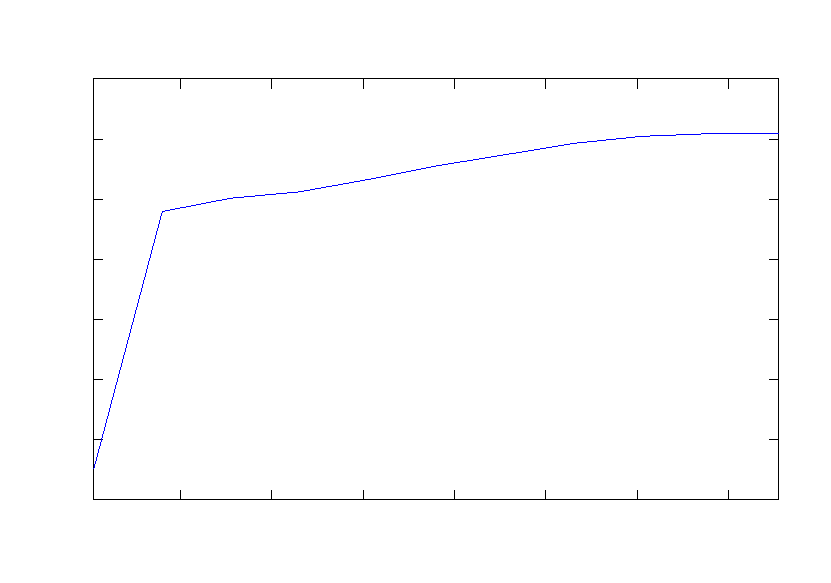
\includegraphics{tasas-vs-imagenes}}%
    \gplfronttext
  \end{picture}%
\endgroup

  \caption{Tasa de aciertos en función de cantidad de imágenes de entrenamiento $n$.}
  \label{tasas-vs-imagenes}
\end{figure}


%%%%%%%%%%%%%%%%%%%%%%%%%%%%%%%%%%%%%%%%%%%%%%%%%%%%%%%%%%%%%%%%%%%%%%%%%%%%%%%
%% Discusión                                                                 %%
%%%%%%%%%%%%%%%%%%%%%%%%%%%%%%%%%%%%%%%%%%%%%%%%%%%%%%%%%%%%%%%%%%%%%%%%%%%%%%%


\section{Discusión}

Observamos una fluctuación en la tasa de aciertos al aumentar el número de iteraciones $i$ del algoritmo QR. Ésta tiende a estabilizarse para valores grandes de $i$. Ver figura \ref{tasas-vs-iteraciones}. Luego de realizar este experimento, decidimos para los siguientes experimentos tomar como criterio de parada la cota de error $e = 1000$, que se alcanza luego de aproximadamente 600 iteraciones.

Observamos un aumento consistente de la tasa de aciertos al incrementar la cantidad de coeficientes principales $k$. Sin embargo, las mejoras en la cantidad de aciertos disminuye considerablemente para valores de $k$ mayores a 40, como se aprecia en la figura \ref{tasas-vs-k}. Esto es de esperar, ya que los coeficientes principales de índices pequeños son los que más información aportan a la imagen.

Verificamos que la tasa de aciertos aumenta uniformemente a medida que se emplean más imágenes para la generación de la matriz de covarianza. Ver fgura \ref{tasas-vs-imagenes}.


%%%%%%%%%%%%%%%%%%%%%%%%%%%%%%%%%%%%%%%%%%%%%%%%%%%%%%%%%%%%%%%%%%%%%%%%%%%%%%%
%% Conclusiones                                                              %%
%%%%%%%%%%%%%%%%%%%%%%%%%%%%%%%%%%%%%%%%%%%%%%%%%%%%%%%%%%%%%%%%%%%%%%%%%%%%%%%


\section{Conclusiones}

Identificamos la configuración $k = 40$, $e = 1000$, que arroja una tasa de aciertos de 82\%, como la configuración óptima para aplicaciones que requieren un uso eficiente del tiempo. Ver figuras \ref{tasas-vs-iteraciones} y \ref{tasas-vs-k}.

Se puede obtener una tasa de aciertos superior aumentando la cantidad de coeficientes principales empleada y reduciendo la cota de error del algoritmo QR si así se desea, pero la mejora es muy pequeña comparado con el tiempo extra de ejecución que requiere. Por ejemplo, la configuración $k = 784$ arroja una tasa de aciertos de 82.03\%, pero requiere el 1960\% del tiempo de ejecución que $k = 40$ (784 vs. 40 productos internos, respectivamente.)

En todos los casos observamos un incremento en la tasa de aciertos al emplear un subconjunto más grande del cuerpo de entrenamiento. Dado que el cuello de botella de este método es la aproximación de autovectores, que es independiente del número de imágenes de entrenamiento empleadas, sugerimos emplear la mayor cantidad de imágenes de entrenamiento posible.

La principal ventaja de este método es su facilidad de implementación. Si disponemos previamente de las aproximaciones de los autovectores de la matriz de covarianza y las transformadas características medias de cada dígito, podemos identificar un dígito manuscrito cualquiera computando $k$ productos internos y 10 normas euclídeas. Sin embargo, la tasa de aciertos que arroja este método es muy pequeña para la mayoría de las aplicaciones: una tasa del 80\% identifica incorrectamente 1 de cada 5 dígitos.

Recomendamos el uso de este método para aplicaciones de baja prioridad y en donde el costo de cometer un error es muy pequeño (ejemplo: identificación de CAPTCHAs\footnote{http://en.wikipedia.org/wiki/CAPTCHA}.) Para aplicaciones críticas recomendamos aplicar técnicas más adecuadas.


%%%%%%%%%%%%%%%%%%%%%%%%%%%%%%%%%%%%%%%%%%%%%%%%%%%%%%%%%%%%%%%%%%%%%%%%%%%%%%%
%% Apéndice A: Enunciado del Trabajo Práctico                                %%
%%%%%%%%%%%%%%%%%%%%%%%%%%%%%%%%%%%%%%%%%%%%%%%%%%%%%%%%%%%%%%%%%%%%%%%%%%%%%%%


\newpage

\section{Apéndice A: Enunciado del Trabajo Práctico}

{\bf Introducci\'on}\\

El reconocimiento \'optico de caracteres (OCR, por sus siglas en ingl\'es) es el proceso por el cual se traducen o convierten im\'agenes de d\'igitos o caracteres (sean \'estos manuscritos o de alguna tipograf\'ia especial) a un formato representable en nuestra computadora (por ejemplo, ASCII). Esta tarea puede ser m\'as sencilla (por ejemplo, cuando tratamos de determinar el texto escrito en una versi\'on escaneada a buena resoluci\'on de un libro) o tornarse casi imposible (recetas indescifrables de m\'edicos, algunos parciales manuscritos de alumnos de m\'etodos num\'ericos, etc).

El objetivo del trabajo pr\'actico es implementar un m\'etodo de reconocimiento de d\'igitos manuscritos basado en la descomposici\'on en valores singulares, y analizar emp\'iricamente los par\'ametros principales del m\'etodo.

Como instancias de entrenamiento, se tiene un conjunto de $n$ im\'agenes de d\'igitos ma\-nus\-cri\-tos en escala de grises del mismo tama\~no y resoluci\'on (varias im\'agenes de cada d\'igito). Cada una de estas im\'agenes sabemos a qu\'e d\'igito se corresponde.
En este trabajo consideraremos la popular base de datos MNIST, utilizada como referencia en esta \'area de investigaci\'on\footnote{\texttt{http://yann.lecun.com/exdb/mnist/}}. 

Para $i = 1,\ldots, n$, sea $x_i \in \real^{m}$ la $i$-\'esima imagen de nuestra base de datos almacenada por filas en un vector, y sea $\mu = (x_1 + \ldots + x_n)/n$ el promedio de las im\'agenes. Definimos $X\in\real^{n\times m}$ como la matriz que contiene en la $i$-\'esima fila al vector $(x_i - \mu)^{t}/\sqrt{n-1}$, y $$X=U \Sigma V^t$$ a su descomposici\'on en valores singulares, con $U\in\real^{n\times n}$ y $V\in\real^{m\times m}$ matrices ortogonales, y $\Sigma\in\real^{n\times m}$ la matriz diagonal conteniendo en la posici\'on $(i,i)$ al $i$-\'esimo valor singular $\sigma_i$.
Siendo $v_i$ la columna $i$ de $V$, definimos para $i = 1,\ldots,n$ la \textsl{transformaci\'on caracter\'istica} del d\'igito $x_{i}$ como el vector $\mathbf{tc}(x_i) = (v_1^t\, x_i, v_2^t\, x_i,\ldots,v_k^t\, x_i) \in\real^k$, donde $k \in\{1,\ldots,m\}$ es un par\'ametro de la implementaci\'on. Este proceso corresponde a extraer las $k$ primeras \textit{componentes principales} de cada imagen. La intenci\'on es que $\mathbf{tc}(x_i)$ resuma la informaci\'on m\'as relevante de la imagen, descartando los detalles o las zonas que no aportan rasgos distintivos.

Dada una nueva imagen $x$ de un d\'igito manuscrito, que no se encuentra en el conjunto inicial de im\'agenes de entrenamiento, el problema de reconocimiento consiste en determinar a qu\'e d\'igito corresponde. Para esto, se calcula $\mathbf{tc}(x)$ y se compara con $\mathbf{tc}(x_i)$, para $i = 1,\ldots, n$. \\

{\bf Enunciado}\\

Se pide implementar un programa que lea desde archivos las im\'agenes de entrenamiento de distintos d\'igitos manuscritos y que, utilizando la descomposici\'on en valores singulares, se calcule la transformaci\'on caracter\'istica de acuerdo con la descripci\'on anterior. Para ello se deber\'a implementar alg\'un m\'etodo de estimaci\'on de autovalores/autovectores. Dada una nueva imagen de un d\'igito manuscrito, el programa deber\'a determinar a qu\'e d\'igito co\-rres\-pon\-de.
El formato de los archivos de entrada y salida queda a elecci\'on del grupo. Si no usan un entorno de desarrollo que incluya bibliotecas para la lectura de archivos de im\'agenes, sugerimos que utilicen im\'agenes en formato \textsc{Raw}. 

Se deber\'an realizar experimentos para medir la efectividad del reconocimiento, analizando tanto la influencia de la cantidad $k$ de componentes principales seleccionadas como la influencia de la precisi\'on en el c\'alculo de los autovalores.\\

{\bf Fecha de entrega} 

\begin{itemize}
\item \textsl{Formato electr\'onico:} viernes 21 de junio de 2013, \underline{hasta las 23:59 hs.}, enviando el trabajo (informe+c\'odigo) a \texttt{metnum.lab@gmail.com}. El subject del email debe comenzar con el texto \verb|[TP3]| seguido de la lista de apellidos de los integrantes del grupo. 
\item \textsl{Formato f\'isico:} lunes 24 de junio de 2013, de 18 a 20hs (en la clase de la pr\'actica).
\end{itemize}


%%%%%%%%%%%%%%%%%%%%%%%%%%%%%%%%%%%%%%%%%%%%%%%%%%%%%%%%%%%%%%%%%%%%%%%%%%%%%%%
%% Apéndice B: Código Fuente                                                 %%
%%%%%%%%%%%%%%%%%%%%%%%%%%%%%%%%%%%%%%%%%%%%%%%%%%%%%%%%%%%%%%%%%%%%%%%%%%%%%%%

\newpage

\section{Apéndice B: Código Fuente}


\subsection{ecuaciones.cpp}

\verbatimtabinput{../ecuaciones.cpp}


\subsection{Matriz.h}

\verbatimtabinput{../Matriz.h}


\subsection{Matriz.cpp}

\verbatimtabinput{../Matriz.cpp}


\subsection{misc.cpp}

\verbatimtabinput{../misc.cpp}


\end{document}